\documentclass{article}
\usepackage{enumitem}
 
 \newlist{FR}{enumerate}{1}
 \setlist[FR]{label=FR-\arabic*:}
\renewcommand{\labelenumii}{\theenumii}
\renewcommand{\theenumii}{\theenumi.\arabic{enumii}.}

\usepackage{graphicx}
\graphicspath{{Figures/}}

\title{Software Requirements Specification}
\date{24 February 2017}
\author{Team Dodger}

\begin{document}
	\pagenumbering{gobble}
	\maketitle
	\newpage
	\tableofcontents
	\newpage
	\pagenumbering{arabic}
	
	\section{Introduction}
	The software requirements specification (SRS) should aptly outline the functional requirements of the system to ensure that a third party could develop the functionality to a required degree without further input. Thus, the functional requirements should be precise and extensive to eliminate deviation from the system’s goals.
	
	\subsection{Purpose}
	The intended audience of the application includes students of the University of Pretoria, the staff and simple visitors. NavUP can be used by new students who do not know their way around campuses yet, or simply by staff members who want to avoid clustered pathways. It is a tool that will help optimise campus navigation and reduce travel time from one destination to the other.
	
	\subsection{Scope}
	The NavUP system will help users to navigate campuses by allowing users to choose destinations, locate their current location, set up the appropriate path by taking into account human congestion and visually representing said path for the user to follow.
	NavUP will have a notifications system that will tell the user of events he/she might be interested in. An achievements system will also be in place to award users for walking certain distances or visiting certain locations.  NavUP also hopes to incorporate locations with access for the disabled into its maps for those that are in need of such features. It will have a timetable feature that will allow users to create personalised timetables which the system could then use to help them get where they need to when they need to. The system will work offline but will lose some of its online features such as notifications for user interests. Users will also be able to broadcast their location so that others can see them on their maps.
	
	\subsection{Definitions, Acronyms and Abbreviations}
	
	\begin{figure}[h!]
		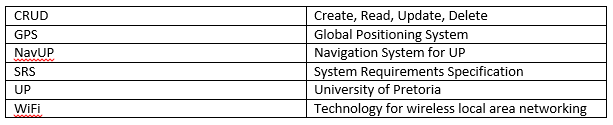
\includegraphics[scale=1]{Descriptions.PNG}
	\end{figure}
	
	\subsection{References}
	\subsection{Overview}
	The SRS will help give a detailed representation of the functional requirements and how the elements of the system interact with eachother to achieve NavUp's purpose. 
	
	\section{Overall Description}
	\subsection{Product Perspective}
		The main system will be a server on campus that is connected to a database where user's details are stored such as degree, interests and timetable. The user will log into the main system by means of a user friendly GUI provided on the mobile application that sends the user's details to the server over the internet to look at the authenticity and correctness of the provided details. Thereafter the main system will load information about the user and populate the GUI with the relevant information based on the category of the current user be it a student or administrator. The application will then use wifi connections, cell phone towers and GPS to determine the user's position and then triangulate them to the destination class or activity based on these calculations. When administrators update the application or database through the server or the application itself it will notify the user and update the relevant information for the user, for example if a class is cancelled, it will update the user's timetable and notify the user of this update through the GUI as well as push notifications. The map of campus can be loaded onto the mobile application to reduce long term internet usage and only the destination and route to get there will be sent over the network.
	\subsection{Product Function}
		\begin{itemize}
 	\item Navigation from and to a location
 	\item Store users timetable to automatically tell user where to go next
	\item View more information about a specific location
 	\item See upcoming events when at a location or based on users interests
 	\item Reward user for completing challenges 
 	\item Update user timetables if classes are cancelled or if there will be a test
 	\end{itemize}
	\subsection{User Characteristics}
	Four categories of users will be present:
 		\begin{itemize}
 
 \item Guest user: Basic education level is needed as this user will just be making use of the navigation system and search system so a basic technical skill will be needed.
 \item Main user (student): This user has at least a high school level education and will be using more advanced parts of the system such as setting up a class timetable, looking at and competing in the reward system and managing their profile.
 \item Administrator / lecturer: This user has at least a high school level education and will need a more advanced technical knowledge as this user will be setting up events, cancelling classes and fixing or updating the system for other users.  
 \item 3rd party Rewards manager: High school level education will be needed as more advanced tasks will be left up to this user such as set up challenges for the other users and include rewards if challenge is completed. An advanced technical knowledge will be needed by this user.
 
 	\end{itemize}
	\subsection{Constraints}
		This section describes restrictions on the options that are available when developing the application within feasable regions.
 		\begin{itemize}
 			\item Connections are limited to different types of networks at different locations. GPS cannot be used within buildings and some buildings lack a strong Wi-Fi signal. Mobile networks may also switch to EDGE in some buildings where faster connections aren't available.
 			\item Application is initially constrained to Android and iOS only.
 			\item Application is designed for approximately 30000 users at any given time which can be seen as a constraint on the number of active users the system can handle.
 			\item The application can experience lengthy response times given that there is a constraint resulting from the capacity of the databases.\newline
 		\end{itemize}
 
	\subsection{Assumptions and Dependencies}
	A major assumption of the NavUP system is related to mobile devices. The first assumption relating to this includes the idea that those who require the services rendered by the application will either have a mobile device or have access to one and have a general knowledge of how to use it. It is also assumed that every users mobile device will have enough memory and performance capabilities in order to run the application. Lastly, it is assumed that these devices will have GPS, WiFi and cellular connectivity capabilities built into the device.
	
	\section{Specific Requirements}
	This section expands on the functional requirements of the system. It gives a detailed 	description of the system and all of its use cases.
	
	\subsection{External Interface Requirements}
		This section provides a detailed description for each interface that composes the system along with other relevant information.
 		\subsubsection{User Interface}
 		\begin{itemize}
 		\item The user interface should initially be a login screen for first time users or logged out users. This login screen will also have the option for new users to register.
 		\item Users should then be able to type in their preferred destination or search via an advanced search method to find a number of different places based on their search criteria.
 		\item A results page will be in the form of a visual map which can be used interactively by the user to view his/her route clearly or to view other places of interest along the way.
 		\item A settings page will be available for users to tweak the application to their needs as well as to update personal settings.\newline
 		\end{itemize}
 		
 		\subsubsection{Hardware Interface}
 		\begin{itemize}
 		\item Abstract interface via application and database infrastructure not visible to user.\newline
 		\end{itemize}
 		
 		\subsubsection{Software Interface}
 		\begin{itemize}
 		\item Application and GPS application communicate in order to receive geographical information. 			\item Application and database communicate in order to receive information about classes and desired locations.\newline
 		\end{itemize}
 		
 		\subsubsection{Communication Interface}
 		\begin{itemize}
 		\item No specific interface implemented. Communication is left to the underlying operating system of the application and portal/database.\newline
 		\end{itemize}
 
	
	\subsection{Functional Requirements}
	This section includes all functional requirements in detail. It includes all use case diagrams, Actor-System interaction diagrams as well as a traceability matrix.	
	\subsubsection{High Level Requirements}
 	\begin{FR}
 		\item The system should have basic navigation functionality 
 		\item The system should be able to provide and visualise information related to pedestrian traffic
 		\item The system should be able to push new information to users based on their preferences and interests
 		\item The system should integrate various activities that use location and movement
 		\item The system should provide functionality to create, read, update and delete users 
 		\item The system should allow users to create and manage timetables
 		\item The system should allow users to save and share locations
 		\item The system should be able to allow users to manage events they are interested in on campus
 	\end{FR}
	\subsubsection{Use cases}
	\begin{enumerate}
		\item \underline{Navigation Subsystem}
			
		
	\begin{enumerate}
		\item Get current location
		\begin{enumerate}
			\item \textbf{Description:} The NavUP system must be able to determine a user’s location at any point in time while the user is on the Hatfield campus. The location must be determined regardless of whether the user is indoors or outdoors.
			\item \textbf{Precondition:} The user must have an active account and must be within range of WiFi routers.
			\item \textbf{Postcondition:} The user’s location is determined and displayed.\newline
		\end{enumerate}
		
		\item Search location
		\begin{enumerate}
			\item \textbf{Description:} The NavUP system must provide functionality that enables a user to search for any location (lecture hall, day-house, restaurant) on the Hatfield Campus.
			\item \textbf{Precondition:} The user must have an active account
			\item \textbf{Postcondition:} Matching locations are returned to the user. If no buildings match the search criteria, an appropriate error message is displayed.\newline
		\end{enumerate}
		
		
		\item View location details
		\begin{enumerate}
			\item \textbf{Description:} The NavUP system must allow users to view details related to specific locations. This could include restaurant menus, lecture hall timetable schedules as well as images of the buildings.
			\item \textbf{Precondition:} The user must have an active account and a valid location must be selected on the map.
			\item \textbf{Postcondition:} Relevant location details shown to user.\newline
		\end{enumerate}
		
		\item View places of interest
		\begin{enumerate}
			\item \textbf{Description:} The NavUP system must be able to display places of interests to a user based on their current location. This will include places like restaurants and day-houses that must be displayed in a list form. 
			\item \textbf{Precondition:} The user must have an active account and their current location must be known.  
			\item \textbf{Postcondition:} Relevant places of interest are listed and displayed to the user based on their location.\newline
		\end{enumerate}
		
		\item Navigate to location
		\begin{enumerate}
			\item \textbf{Description:} The NavUP system must be able to provide directions and navigate to a location given the user’s current location as well as a desired destination. The system should calculate the most optimal route by looking at the shortest path as well as pedestrian traffic.
			\item \textbf{Precondition:} The user must have an active account. The user’s current location must be known and the must have specified a destination through the search interface.
			\item \textbf{Postcondition:} The user is provided with directions from their current location to their desired destination.\newline
		\end{enumerate}
		
		\item Show pedestrian traffic
		\begin{enumerate}
			\item \textbf{Description:} The NavUP system must be able to display pedestrian traffic on campus in the form of a heatmap. When navigating to a specified location, the system must show traffic on that specific route. A user should also be able to view an overall heatmap of the campus to see traffic.
			\item \textbf{Precondition:} Users must all have the NavUP app installed and must be registered in order for them to show up on the heatmap.
			\item \textbf{Postcondition:} A heatmap of the campus is displayed. 
		\end{enumerate}
	\end{enumerate}
	\begin{figure}[h!]
		\includegraphics[scale=0.5]{Navigation_Subsystem.png}
		\caption{Navigation Subsystem}	
	\end{figure}
	
	\subsection{Get Current Location}
	
	\begin{tabular}{ | m{15em} | m{15em}| } 
		\hline
		Preconditions: 							& The user must have an active account and must be within range of WiFi routers. \\
		\hline
		Actor: User 								&  System: Up Nav \\ 
		\hline
											& 0. The system  displays the user's Home page\\ 
		\hline
		1. The user selects the "Navigation" option			& 2. The system displays the Navigation page. \\
		\hline
		3. The user selects the "Get Current Location" option. 	& 4. The system determines the users current location. \\
		\hline																
											& 5. The system displays a map on which the users current location is presented. \\
		\hline
		Post Conditions: 							& The users location is determined and displayed. \\
		\hline
	\end{tabular}

	\subsection{Search Location}
	\begin{tabular}{ | m{15em} | m{15em}| } 
		\hline
		Preconditions: 													& The user must have an active account \\
		\hline
		Actor: User 														&  System: Up Nav \\ 
		\hline
																	& 0. The system  displays the user's Home page\\ 
		\hline
		1. The user selects the "Navigation" option									& 2. The system displays the Navigation page. \\
		\hline
		3. The user selects the "Search Location" option.								& 4. The system displays a search bar on the screen. \\ 
		\hline
		5. The User enters a location which they would like to search for and press the search button		& 6. The system searches all the registered locations based on the search term entered by the user. \\
		\hline
																	& 7. The system displays a list of locations which matched the search criteria. \\
		\hline
		Post Conditions:													&Matching locations are returned to the user. If no buildings match the search criteria, an appropriate error message is displayed. \\
		\hline
	\end{tabular}

	\subsection{View Location Details}
	
		\begin{tabular}{ | m{15em} | m{15em}| } 
		\hline
		Preconditions                                                     					& The user must have an active account and a valid location must be selected on the map. \\ 
		\hline
		Actor: User                                                      					& System: Up Nav  \\ 
		\hline
                                                                 							& 0. The system displays a list of locations from the location search.  \\
		 \hline
		1. The user selects one of the locations from the provided list. 		& 2. The system retrieves information related to the location selected by the user. \\ 
		\hline
                                                                 							& 3. The system displays the location information. \\ 
		\hline
		Post conditions									& Relevant location details shown to user. \\
		\hline
		\end{tabular}

	\subsection{View Places of Interest}
	
	\centering
		\begin{tabular}{ | m{15em} | m{15em}| }
		\hline
		Preconditions                                             				& The user must have an active account and their current location must be known. \\ 
		\hline
		Actor: User                                              				& System: Up Nav \\
		 \hline
                                                          							& 0. The system displays the user's Home page. \\
		\hline
		1. The user selects the "Navigation" option				& 2. The system displays the Navigation page. \\
		\hline
		3. The user selects the "View Places of Interest" option. 		& 4. The system retrieves a list of general places of interest based on the user's location. \\ 
		\hline
                                                          							& 5. The system displays the places of interest to the user. \\ 
		\hline
		Post conditions								& Relevant location details shown to user. \\
		\hline
		\end{tabular}

	\subsection{Navigate to Location}

	\centering

	\begin{tabular}{ | m{15em} | m{15em}| }
		\hline 
		Preconditions                                                                                 						& The user must have an active account. The users current location must be known and the must have specified a destination through the search interface. \\ 
		\hline
		Actor: User                                                                                  						& System: Up Nav \\ 
		\hline
                                                                                             									& 0. The system displays the details of a location. \\ 
		\hline
		1. The user selects the "Navigate to Location" option                                        				& 2. The system displays a list of navigation preferences for the user to enable / disable, namely "Avoid Pedestrian Traffic" and "Disability Friendly Route". \\
		\hline
		3. The user selects their desired preferences.                                               				& 4. The system calculates a route based on the user's preferences. \\ 
		\hline
                                                                                            									& 5. The system marks the calculated route on the map and displays this map to the user. \\ 
		\hline
																	& 6. UC 1.6 View Pedestrian Traffic \\
		\hline
		Post conditions                                                                               						& The user is provided with directions from their current location to their desired destination \\ 
		\hline
	\end{tabular}
	
	\subsection{View Pedestrian Traffic}
	\begin{tabular}{ | m{15em} | m{15em}| }
		\hline
		Preconditions													& Users must all have the NavUP app installed and must be registered in order for them to show up on the heat map. The current user must have selected the option to navigate to a location \\
		\hline
		Actor: User														& System: Up Nav \\
		\hline
																	& 0. The system scans the calculated route for other users. \\
		\hline
																	& 1. The system displays a heat map to indicate the amount of users along the selected route. \\
		\hline
		Post condition													& A heat map of the campus is displayed \\
		\hline

	\end{tabular}

	
	\begin{table}[h!]
\centering
\caption{Navigation Subsystem Traceability Matrix}
\label{my-label}
\begin{tabular}{cc|c|c|c|c|c|c|}
\cline{3-8}
                                           &                   & \multicolumn{6}{c|}{\textbf{Use Cases}} \\ \hline
\multicolumn{1}{|c|}{\textbf{Requirement}} & \textbf{Priority} & 1.1  & 1.2  & 1.3  & 1.4  & 1.5  & 1.6  \\ \hline
\multicolumn{1}{|c|}{FR-1}                 & 1                 & X    & X    &      &      & X    & X    \\ \hline
\multicolumn{1}{|c|}{FR-2}                 & 5                 &      &      &      &      &      & X    \\ \hline
\multicolumn{1}{|c|}{FR-3}                 & 7                 & X    & X    &      &      &      &      \\ \hline
\multicolumn{1}{|c|}{FR-4}                 & 8                 & X    &      &      &      & X    &      \\ \hline
\multicolumn{1}{|c|}{FR-5}                 & 2                 &      &      &      &      &      &      \\ \hline
\multicolumn{1}{|c|}{FR-6}                 & 4                 &      &      &      &      &      &      \\ \hline
\multicolumn{1}{|c|}{FR-7}                 & 3                 &      & X    &      &      &      &      \\ \hline
\multicolumn{1}{|c|}{FR-8}                 & 6                 &      & X    &      & X    &      &      \\ \hline
\multicolumn{2}{|c|}{\textbf{Use Case Priority}}               & 1    & 3    & 4    & 6    & 2    & 5    \\ \hline
\end{tabular}
\end{table}



\begin{table}[]
\centering
\caption{Location Management Subsystem Traceability Matrix}
\label{my-label}
\begin{tabular}{cc|c|c|c|c|c|}
\cline{3-7}
                                           &                   & \multicolumn{5}{c|}{\textbf{Use Cases}} \\ \hline
\multicolumn{1}{|c|}{\textbf{Requirement}} & \textbf{Priority} & 2.1    & 2.2    & 2.3   & 2.4   & 2.5   \\ \hline
\multicolumn{1}{|c|}{FR-1}                 & 1                 &        & X      & X     &       & X     \\ \hline
\multicolumn{1}{|c|}{FR-2}                 & 5                 &        &        &       &       &       \\ \hline
\multicolumn{1}{|c|}{FR-3}                 & 7                 & X      &        &       &       & X     \\ \hline
\multicolumn{1}{|c|}{FR-4}                 & 8                 &        &        &       & X     &       \\ \hline
\multicolumn{1}{|c|}{FR-5}                 & 2                 &        &        &       &       &       \\ \hline
\multicolumn{1}{|c|}{FR-6}                 & 4                 &        &        &       &       &       \\ \hline
\multicolumn{1}{|c|}{FR-7}                 & 3                 & X      & X      &       & X     &       \\ \hline
\multicolumn{1}{|c|}{FR-8}                 & 6                 &        &        & X     &       &       \\ \hline
\multicolumn{2}{|c|}{\textbf{Use Case Priority}}               & 1      & 4      & 5     & 2     & 3     \\ \hline
\end{tabular}
\end{table}

\section{User Account Management System}

	\subsection{Create Profile}

	\centering

	\begin{tabular}{ | m{15em} | m{15em}| }
		\hline
		Preconditions                                                       				& The user must not exist on the system \\ 				
		\hline
		Actor: User                                                       					& System: Up Nav \\ 			
		\hline
                                                                  							& 0. The system displays Login Page with a "Register" option. \\                                                           
		 \hline
		1. The user selects the "Register" option.					& 2.  The system displays a form for the user to complete their profile. \\				
		\hline
		3. The user fills in their profile details and selects the save option. 		& 4. The system saves the users profile details and notifies the user that their profile has been created. \\ 
		\hline
		Post condition                                                     				& The new user is registered on the system \\ 				
		\hline
	\end{tabular}

	\subsection{Login}
	
	\centering
	\begin{tabular}{ | m{15em} | m{15em}| }
		\hline
		Preconditions                                    												& The user must be registered on the system \\ 
		\hline
		Actor: User                                     												& System: Up Nav \\ 
		\hline
                                               		 													& 0. The system displays the user's Login page. \\ 
		\hline
		1. The user enters their username and password. 										& 2. The system verifies the credentials entered by the user. \\
		\hline
                                                															& 3. The system logs the user in and displays the user's home page. \\
		\hline
		Post condition                                  												& The user is logged in to the system \\ 
		\hline
	\end{tabular}


	\subsection{Manage Profile}
	\begin{tabular}{ | m{15em} | m{15em}| }
		\hline
		Preconditions                                                       						& The user must be logged in \\ 				
		\hline
		Actor: User                                                       							& System: Up Nav \\ 			
		\hline
                                                                  									& 0. The system displays the user's Home page. \\                                                           
		 \hline
		1. The user selects the "Manage Account" option.						& 2. The system displays the User Account Management page. \\
		 \hline
		3. The user selects the "Manage Profile" option. 						& 4.  The system displays a form which is populated by the users current profile details. \\
		\hline
		5a. The user edits their current details and selects the save option. 			& 6a. The system saves the users profile details and notifies the user that their details have been saved. \\ 
		\hline
		5b. The user selects the "Delete Profile" option.						& 6b The system prompts the user to confirm the deletion. \\
		\hline
		7b The user confirms the deletion.								& 8b. The system deletes the users profile and notifies the user that their profile has been deleted. \\
		\hline
		Post condition                                                     						& None \\ 			
		\hline
	\end{tabular}

	\subsection{Create Timetable}
	\begin{tabular}{ | m{15em} | m{15em}| }
		\hline
		Preconditions                                                       				& The user must be logged in \\ 				
		\hline
		Actor: User                                                       					& System: Up Nav \\ 			
		\hline
                                                                  							& 0. The system displays the user's Home page. \\                                                           
		 \hline
		1. The user selects the "Manage Account" option.				& 2. The system displays the User Account Management page. \\
		 \hline
		3. The user selects the "Create Timetable" option. 				& 4.  The system displays a timetable for the user to complete. \\
		\hline
		5a. The user adds their lecture details on the timetable. 			& 6a. The system saves the timetable and notifies the user that their timetable has been saved. \\ 
		\hline
		Post condition                                                     				& A new timetable is created for the user. \\ 			
		\hline
	\end{tabular}

	\subsection{Manage Timetable}
	\begin{tabular}{ | m{15em} | m{15em}| }
		\hline
		Preconditions                                                       				& The user must be logged in \\ 				
		\hline
		Actor: User                                                       					& System: Up Nav \\ 			
		\hline
                                                                  							& 0. The system displays the user's home page. \\                                                           
		 \hline
		1. The user selects the "Manage Account" option.				& 2. The system displays the User Account Management page. \\
		 \hline
		3. The user selects the "Manage Timetable" option. 				& 4.  The system displays the user's current timetable. \\
		\hline
		5a. The user edits their current timetable and selects the save option. 	& 6a. The system saves the users timetable and notifies the user that their timetable have been saved. \\ 
		\hline
		5b. The user selects the "Delete Timetable"  option.				&6b. The system deletes the user's timetable  and notifies the user that their timetable has been deleted. \\
		\hline
		Post condition                                                     				& The user's timetable is edited or deleted \\ 			
		\hline
	\end{tabular}



\begin{table}
\centering
\caption{User Account Management Subsystem Traceability Matrix}
\label{my-label}
\begin{tabular}{|c|c|c|c|c|c|c|}
\hline
\multicolumn{2}{|c|}{}                           & \multicolumn{5}{c|}{\textbf{Use Cases}}                                  \\ \hline
\textbf{Requirement}     & \textbf{Priority}     & \textbf{2.1} & \textbf{2.2} & \textbf{2.3} & \textbf{2.4} & \textbf{2.5} \\ \hline
\textbf{FR-1}            & \textbf{1}            & \textbf{}    & \textbf{}    & \textbf{}    & \textbf{}    & \textbf{}    \\ \hline
\textbf{FR-2}            & \textbf{5}            & \textbf{}    & \textbf{}    & \textbf{}    & \textbf{}    & \textbf{}    \\ \hline
\textbf{FR-3}            & \textbf{7}            & \textbf{}    & \textbf{}    & \textbf{}    & \textbf{}    & \textbf{}    \\ \hline
\textbf{FR-4}            & \textbf{8}            & \textbf{}    & \textbf{}    & \textbf{}    & \textbf{}    & \textbf{}    \\ \hline
\textbf{FR-5}            & \textbf{2}            & \textbf{X}   & \textbf{X}   & \textbf{X}   & \textbf{}    & \textbf{}    \\ \hline
\textbf{FR-6}            & \textbf{4}            & \textbf{}    & \textbf{}    & \textbf{}    & \textbf{X}   & \textbf{X}   \\ \hline
\textbf{FR-7}            & \textbf{3}            & \textbf{}    & \textbf{}    & \textbf{}    & \textbf{}    & \textbf{}    \\ \hline
\textbf{FR-8}            & \textbf{6}            & \textbf{}    & \textbf{}    & \textbf{}    & \textbf{}    & \textbf{}    \\ \hline
\multicolumn{2}{|c|}{\textbf{Use Case Priority}} & \textbf{1}   & \textbf{2}   & \textbf{3}   & \textbf{4}   & \textbf{5}   \\ \hline
\end{tabular}
\end{table}	

\begin{table}[]
\centering
\caption{Entertainment Subsystem Traceability Matrix}
\label{my-label}
\begin{tabular}{|c|c|c|c|c|l|l|}
\hline
\multicolumn{2}{|c|}{}                           & \multicolumn{5}{c|}{\textbf{Use Cases}}                           \\ \hline
\textbf{Requirement}     & \textbf{Priority}     & \textbf{4.1}  & \textbf{4.2}  & \multicolumn{3}{c|}{\textbf{4.3}} \\ \hline
\textbf{FR-1}            & \textbf{1}            & \textbf{X}    & \textbf{}     & \multicolumn{3}{c|}{\textbf{}}    \\ \hline
\textbf{FR-2}            & \textbf{5}            & \textbf{}     & \textbf{}     & \multicolumn{3}{c|}{\textbf{}}    \\ \hline
\textbf{FR-3}            & \textbf{7}            & \textbf{}     & \textbf{}     & \multicolumn{3}{c|}{\textbf{}}    \\ \hline
\textbf{FR-4}            & \textbf{8}            & \textbf{}     & \textbf{}     & \multicolumn{3}{c|}{\textbf{}}    \\ \hline
\textbf{FR-5}            & \textbf{2}            & \textbf{}     & \textbf{}     & \multicolumn{3}{c|}{\textbf{}}    \\ \hline
\textbf{FR-6}            & \textbf{4}            & \textbf{}     & \textbf{}     & \multicolumn{3}{c|}{\textbf{}}    \\ \hline
\textbf{FR-7}            & \textbf{3}            & \textbf{}     & \textbf{X}    & \multicolumn{3}{c|}{\textbf{}}    \\ \hline
\textbf{FR-8}            & \textbf{6}            & \textbf{X}    & \textbf{X}    & \multicolumn{3}{c|}{\textbf{X}}   \\ \hline
\multicolumn{2}{|c|}{\textbf{Use Case Priority}} & \textbf{1}    & \textbf{2}    & \multicolumn{3}{c|}{\textbf{3}}   \\ \hline
\end{tabular}
\end{table}
	
	\item \underline{Location Management Subsystem}
\begin{enumerate}
		\item Save Location
		\begin{enumerate}
			\item \textbf{Description:} The NavUP system must be able to save a location that the user specifies. 
			\item \textbf{Precondition:} User must be logged in if they want to save locations, and be in range of WiFi.
			\item \textbf{Postcondition:} A location will be saved to the users profile.\newline
		\end{enumerate}
		
		\item View Saved Location 
		\begin{enumerate}
			\item \textbf{Description:} The NavUP system must allow users to view locations that the user has saved to their profile. 
			\item \textbf{Precondition:} The user must be logged in and be in range of WiFi.
			\item \textbf{Postcondition:} None.\newline
		\end{enumerate}
		
		\item View History 
		\begin{enumerate}
			\item \textbf{Description:} The NavUP system should be able to allow users to view their history of locations.
			\item \textbf{Precondition:} The user must be logged in and be in range of WiFi.
			\item \textbf{Postcondition:} None.\newline
		\end{enumerate}
		
		\item Share Location  
		\begin{enumerate}
			\item \textbf{Description:} The NavUP system should provide the users with a means to share their current location so as to allow other users to know where they are. 
			\item \textbf{Precondition:} The user must be logged in and be in range of WiFi.
			\item \textbf{Postcondition:} User location is broadcasted for other users to see.\newline
		\end{enumerate}
		
		\item View Most Visited Locations  
		\begin{enumerate}
			\item \textbf{Description:} The NavUP system should have a favourite location section which can then be accessed by the user to view their most visited areas. 
			\item \textbf{Precondition:} The user must be logged in and be in range of WiFi.
			\item \textbf{Postcondition:} None.\newline
		\end{enumerate}
	\end{enumerate}
	\begin{figure}[h!]
		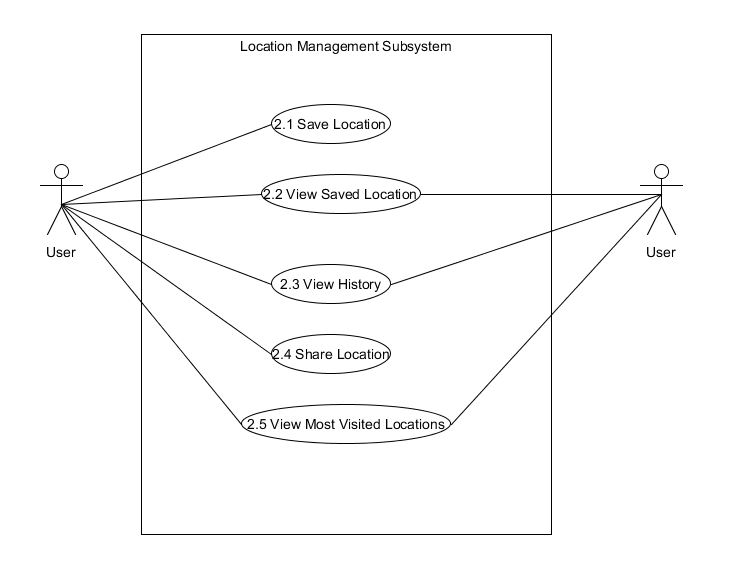
\includegraphics[scale=0.5]{Location_Management.JPG}
		\caption{Location Management Subsystem}	
	\end{figure}
	
	\section{Location Sub-System}

	\subsection{Save Location}

	\centering

	\begin{tabular}{ | m{15em} | m{15em}| }
		\hline
		Preconditions                                    										& The user must be logged in to the system.  \\ 
		\hline
		Actor: User                                     										& System: Up Nav                                                                  \\ 
		\hline
                                               													& 0. The system displays the details of a location which was selected by the user \\
		\hline
		1. The user selects the "Save Location" option. 								& 2. The system adds the location to the "Saved Locations" list. \\
		\hline
                                                													& 3. The system notifies the user that the location has been saved. \\
		\hline
		Post condition                                   										& The location will be saved to the user's Saved Locations list \\
		\hline
	\end{tabular}
	
	\subsection{View Saved Locations}

	\centering

	\begin{tabular}{ | m{15em} | m{15em}| }
		\hline
		Preconditions                                          										& The user must be logged in \\ 
		\hline
		Actor: User                                            										& System: Up Nav \\
		\hline
                                                       												& 0. The system displays the user's Home page. \\ 
		\hline
		1. The user selects the "Manage Locations" option								& 2. The system displays the Manage Locations page. \\
		\hline
		3. The user selects the "View Saved Locations" option.							& 4. The system retrieves a list of all the locations previously saved by the user. \\ 
		\hline
                                                      												& 5. The system displays a list of saved locations. \\
		\hline
		Post condition                                         		 								& None                                                                              \\
		\hline
	\end{tabular}


	\subsection{View History}

	\centering

	\begin{tabular}{ | m{15em} | m{15em}| }
		\hline
		Preconditions                                   										& The user must be logged in \\ 
		\hline
		Actor: User                                    										& System: Up Nav \\ 
		\hline
                                               													& 0. The system displays the user's Home page. \\ 
		\hline
		1. The user selects the "Manage Locations" option								& 2. The system displays the Manage Locations page. \\
		\hline
		3. The user selects the "View History" option. 									& 4. The system retrieves a list of all the locations previously searched for by the user. \\ 
		\hline
                                               													& 5. The system displays a list of the user's history. \\
		 \hline
		Post condition                                 										& None \\ 
		\hline
	\end{tabular}
	

	\subsection{Share Location}

	\centering

	\begin{tabular}{ | m{15em} | m{15em}| }
		\hline
		Preconditions                                                                                                						& The user must select the "View Current Location" option \\ 
		\hline
		Actor: User                                                                                                						 	& System: Up Nav \\ 
		\hline
                                                                                                            									& 0. The system displays the user's current location. \\ 
		\hline
		1. The user selects the "Share Location" option.                                                            					& 2. The system displays a search bar to search for users. \\
		\hline
		3. The user enters the user name of the user they wish to send a location to and presses the search button. 	& 4. The system searches for the user based on the search term entered by the user. \\ 
		\hline
                                                                                                            									& 5. The system displays the search results. \\ 
		\hline
		6. The user selects the user which they would like to share their location with.                            			& 7. The system sends a location to the selected user. \\ 
		\hline
		Post condition                                                                                               						& The current user's location is sent to another user. \\ 
		\hline

	\end{tabular}


	\subsection{View Most Visited Locations}

	\centering

		\begin{tabular}{ | m{15em} | m{15em}| }
		\hline
		Preconditions                                                  											& The user must be logged in \\ 
		\hline
		Actor: User                                                  											& System: Up Nav \\ 
		\hline
                                                              														& 0. The system displays the user's Home page. \\ 
		\hline
		1. The user selects the "Manage Locations" option										& 1. The system displays the Manage Locations page. \\
		\hline
		3. The user selects the "View Most Visited Locations" option. 								& 3. The system retrieves a list of the user's visited locations ordered by frequency of navigation. \\ 
		\hline
                                                              														& 5. The system displays the list of visited locations to the user. \\ 
		\hline
		Post condition                                                											& The user's most visited locations are displayed \\ 
		\hline
	\end{tabular}

	
	\item \underline{User Account Management Subsystem}
	\begin{enumerate}
		\item Create Profile
		\begin{enumerate}
			\item \textbf{Description:} The NavUP system must be able to provide the user with a means to create their profiles which will then allow them to login to the NavUP application. 
			\item \textbf{Precondition:} User must be in range of WiFi.
			\item \textbf{Postcondition:} A new user account is created.\newline
		\end{enumerate}
		
		\item Login Function
		\begin{enumerate}
			\item \textbf{Description:} The NavUP system must allow users with a profile to be able to login to said profile and use the NavUP system to the fullest. 
			\item \textbf{Precondition:} User must be in range of WiFi and have an existing NavUP account.
			\item \textbf{Postcondition:} User is logged in.\newline
		\end{enumerate}
		
		\item Manage Profile
		\begin{enumerate}
			\item \textbf{Description:} The NavUP system must allow users to manage their own profiles as well as allow administrators to keep track of user profiles. 
			\item \textbf{Precondition:} User must be in range of WiFi and logged in. Admin has no precondition.  
			\item \textbf{Postcondition:} User profile may be altererd.\newline
		\end{enumerate}
		
		\item Create Timetable
		\begin{enumerate}
			\item \textbf{Description:} The NavUP system should be able to allow users to create their personal timetables. 
			\item \textbf{Precondition:} User must be in range of WiFi and logged in.
			\item \textbf{Postcondition:} Timetable is created on user's profile.\newline
		\end{enumerate}
		
		\item Manage Timetable
		\begin{enumerate}
			\item \textbf{Description:} The NavUP system must allow users to edit or manage their existing timetables so as to fit their needs. It must also allow administrators to keep track of the user’s timetable. 
			\item \textbf{Precondition:} User must have existing timetable.
			\item \textbf{Postcondition:} Timetable is edited on the users profile.\newline
		\end{enumerate}
	\end{enumerate}
	\begin{figure}[h!]
		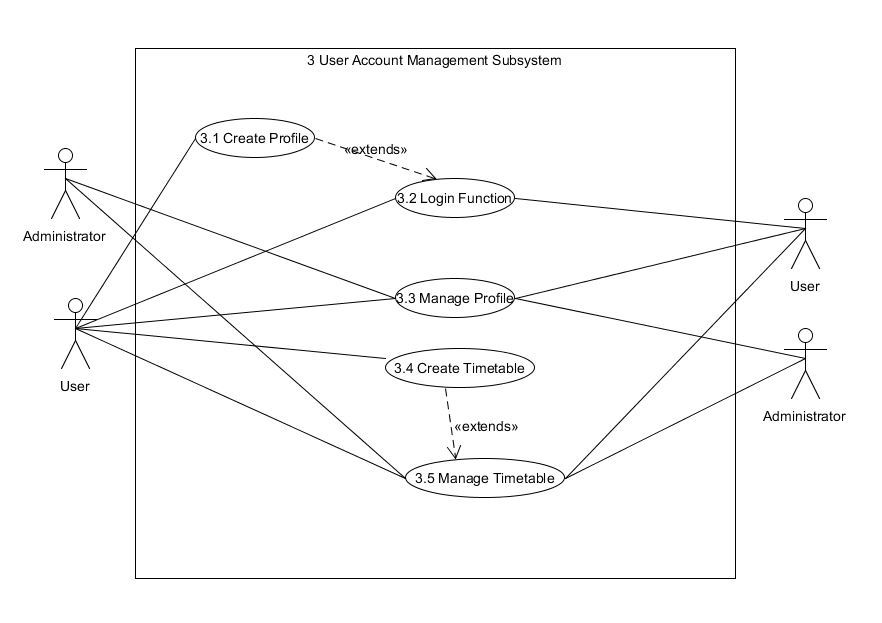
\includegraphics[scale=0.5]{User_Account_Management.JPG}
		\caption{User Account Management Subsystem}	
	\end{figure}
	
		\section{User Account Management System}

	\subsection{Create Profile}

	\centering

	\begin{tabular}{ | m{15em} | m{15em}| }
		\hline
		Preconditions                                                       				& The user must not exist on the system \\ 				
		\hline
		Actor: User                                                       					& System: Up Nav \\ 			
		\hline
                                                                  							& 0. The system displays Login Page with a "Register" option. \\                                                           
		 \hline
		1. The user selects the "Register" option.					& 2.  The system displays a form for the user to complete their profile. \\				
		\hline
		3. The user fills in their profile details and selects the save option. 		& 4. The system saves the users profile details and notifies the user that their profile has been created. \\ 
		\hline
		Post condition                                                     				& The new user is registered on the system \\ 				
		\hline
	\end{tabular}

	\subsection{Login}
	
	\centering
	\begin{tabular}{ | m{15em} | m{15em}| }
		\hline
		Preconditions                                    												& The user must be registered on the system \\ 
		\hline
		Actor: User                                     												& System: Up Nav \\ 
		\hline
                                               		 													& 0. The system displays the user's Login page. \\ 
		\hline
		1. The user enters their username and password. 										& 2. The system verifies the credentials entered by the user. \\
		\hline
                                                															& 3. The system logs the user in and displays the user's home page. \\
		\hline
		Post condition                                  												& The user is logged in to the system \\ 
		\hline
	\end{tabular}


	\subsection{Manage Profile}
	\begin{tabular}{ | m{15em} | m{15em}| }
		\hline
		Preconditions                                                       						& The user must be logged in \\ 				
		\hline
		Actor: User                                                       							& System: Up Nav \\ 			
		\hline
                                                                  									& 0. The system displays the user's Home page. \\                                                           
		 \hline
		1. The user selects the "Manage Account" option.						& 2. The system displays the User Account Management page. \\
		 \hline
		3. The user selects the "Manage Profile" option. 						& 4.  The system displays a form which is populated by the users current profile details. \\
		\hline
		5a. The user edits their current details and selects the save option. 			& 6a. The system saves the users profile details and notifies the user that their details have been saved. \\ 
		\hline
		5b. The user selects the "Delete Profile" option.						& 6b The system prompts the user to confirm the deletion. \\
		\hline
		7b The user confirms the deletion.								& 8b. The system deletes the users profile and notifies the user that their profile has been deleted. \\
		\hline
		Post condition                                                     						& None \\ 			
		\hline
	\end{tabular}

	\subsection{Create Timetable}
	\begin{tabular}{ | m{15em} | m{15em}| }
		\hline
		Preconditions                                                       				& The user must be logged in \\ 				
		\hline
		Actor: User                                                       					& System: Up Nav \\ 			
		\hline
                                                                  							& 0. The system displays the user's Home page. \\                                                           
		 \hline
		1. The user selects the "Manage Account" option.				& 2. The system displays the User Account Management page. \\
		 \hline
		3. The user selects the "Create Timetable" option. 				& 4.  The system displays a timetable for the user to complete. \\
		\hline
		5a. The user adds their lecture details on the timetable. 			& 6a. The system saves the timetable and notifies the user that their timetable has been saved. \\ 
		\hline
		Post condition                                                     				& A new timetable is created for the user. \\ 			
		\hline
	\end{tabular}

	\subsection{Manage Timetable}
	\begin{tabular}{ | m{15em} | m{15em}| }
		\hline
		Preconditions                                                       				& The user must be logged in \\ 				
		\hline
		Actor: User                                                       					& System: Up Nav \\ 			
		\hline
                                                                  							& 0. The system displays the user's home page. \\                                                           
		 \hline
		1. The user selects the "Manage Account" option.				& 2. The system displays the User Account Management page. \\
		 \hline
		3. The user selects the "Manage Timetable" option. 				& 4.  The system displays the user's current timetable. \\
		\hline
		5a. The user edits their current timetable and selects the save option. 	& 6a. The system saves the users timetable and notifies the user that their timetable have been saved. \\ 
		\hline
		5b. The user selects the "Delete Timetable"  option.				&6b. The system deletes the user's timetable  and notifies the user that their timetable has been deleted. \\
		\hline
		Post condition                                                     				& The user's timetable is edited or deleted \\ 			
		\hline
	\end{tabular}
	
	
	\item \underline{Entertainment Subsystem}
			\begin{enumerate}
		\item View events
		\begin{enumerate}
			\item \textbf{Description:} The NavUP system must enable users to view all events that are happening around campus in chronological order. The system should suggest events to a user based on their preferences and most visited locations.
			\item \textbf{Precondition:} The user must have an active account and must be logged in.
			\item \textbf{Postcondition:} Various campus-wide events are returned to the user.\newline
		\end{enumerate}
		
		\item Save event
		\begin{enumerate}
			\item \textbf{Description:} The NavUP system must enable users to save events that they are interested so that they can be viewed later.
			\item \textbf{Precondition:} The user must have an active account, must be logged in and there must be events available to save.
			\item \textbf{Postcondition:} An event is saved.\newline
		\end{enumerate}
		
		\item Delete event
		\begin{enumerate}
			\item \textbf{Description:} The NavUP system must enable a user to delete any saved events
			\item \textbf{Precondition:} The user must have an active account, must be logged in and must have saved events
			\item \textbf{Postcondition:} A saved event is deleted .\newline
		\end{enumerate}
	\end{enumerate}
	\begin{figure}[h!]
		\includegraphics[scale=0.5]{Entertainment_Subsystem.png}
		\caption{Navigation Subsystem}	
	\end{figure}	
	
	\section{Entertainment Sub-System}
	
	\subsection{View Events}
	\begin{tabular}{ | m{15em} | m{15em}| }
		\hline
		Preconditions                                                       				& The user must be logged in \\ 				
		\hline
		Actor: User                                                       					& System: Up Nav \\ 			
		\hline
                                                                  							& 0. The system displays the user's Home page. \\                                                           
		 \hline
		1. The user selects the "Entertainment" option.				& 2. The system displays the Entertainment  page. \\
		 \hline
		3. The user selects the "View Events" option. 					& 4.  The system retrieves a list of all scheduled events . \\
		\hline
													& 5. The system displays the list of events. \\
		\hline
		Post condition                                                     				& A list of all events is displayed to the user \\ 			
		\hline
	\end{tabular}
	
	\subsection{Save Event}
	\begin{tabular}{ | m{15em} | m{15em}| }
		\hline
		Preconditions                                                       				& The user has selected the View Events option \\ 				
		\hline
		Actor: User                                                       					& System: Up Nav \\ 			
		\hline
                                                                  							& 0. The system displays the list of all scheduled events. \\                                                           
		 \hline
		1. The user selects an event from the list.					& 2. The system displays the details of the event selected by the user. \\
		 \hline
		3. The user selects the "Save Event" option. 					& 4.  The system saves the event on the user's "Upcoming Events" list and notifies the user that the event has been saved . \\
		\hline
		Post condition                                                     				& An event is saved on the user's Upcoming Events list \\ 			
		\hline
	\end{tabular}

	\subsection{Delete Event}
	\begin{tabular}{ | m{15em} | m{15em}| }
		\hline
		Preconditions                                                       											& None \\ 				
		\hline
		Actor: User                                                       												& System: Up Nav \\ 			
		\hline
                                                                  														& 0. The system displays the user's Home page. \\                                                           
		 \hline
		1. The user selects the "Entertainment" option.											& 2. The system displays the Entertainment  page. \\
		 \hline
		3. The user selects the "Manage Events" option. 											& 4.  The system retrieves a list of all the user's "Upcoming  Events" . \\
		\hline
		5. The user selects an event from their Upcoming Events list that they wish to delete.						& 6. The system prompts the user to confirm the deletion. \\
		\hline
		7. The user confirms the deletion														& 8. The system removes the event from their Upcoming Events list \\
		\hline
		Post condition                                                     											& An event is removed from the user's Upcoming Event list \\ 			
		\hline
	\end{tabular}
	
	\item \underline{Achievements Subsystem}
	\begin{table}[]
 \centering
 \caption{Achievements Subsystem Traceability Matrix}
 \label{my-label}
 \begin{tabular}{cc|c|c|c|c|}
 \cline{3-6}
                                   &          & \multicolumn{4}{c|}{Use Cases} \\ \hline
 \multicolumn{1}{|c|}{Requirement} & Priority & 5.1    & 5.2   & 5.3   & 5.4   \\ \hline
 \multicolumn{1}{|c|}{FR-1}        & 1        &        &       &       &       \\ \hline
 \multicolumn{1}{|c|}{FR-2}        & 5        &        &       &       &       \\ \hline
 \multicolumn{1}{|c|}{FR-3}        & 7        & X      & X     &       & X     \\ \hline
 \multicolumn{1}{|c|}{FR-4}        & 8        & X      & X     & X     & X     \\ \hline
 \multicolumn{1}{|c|}{FR-5}        & 2        &        &       &       &       \\ \hline
 \multicolumn{1}{|c|}{FR-6}        & 4        &        &       &       &       \\ \hline
 \multicolumn{1}{|c|}{FR-7}        & 3        &        &       & X     &       \\ \hline
 \multicolumn{1}{|c|}{FR-8}        & 6        &        &       &       &       \\ \hline
 \multicolumn{2}{|c|}{Use Case Priority}      & 2      & 3     & 1     & 3     \\ \hline
 \end{tabular}
 \end{table}
	\item \underline{Administration Subsystem}
			\begin{table}[]
 \centering
 \caption{Administration Subsystem Traceability Matrix}
 \label{my-label}
 \begin{tabular}{cc|c|c|c|c|}
 \cline{3-6}
                                   &          & \multicolumn{4}{c|}{Use Cases} \\ \hline
 \multicolumn{1}{|c|}{Requirement} & Priority & 6.1    & 6.2   & 6.3   & 6.4   \\ \hline
 \multicolumn{1}{|c|}{FR-1}        & 1        &        &       &       &       \\ \hline
 \multicolumn{1}{|c|}{FR-2}        & 5        &        &       &       &       \\ \hline
 \multicolumn{1}{|c|}{FR-3}        & 7        &        &       &       & X     \\ \hline
 \multicolumn{1}{|c|}{FR-4}        & 8        &        & X     &       &       \\ \hline
 \multicolumn{1}{|c|}{FR-5}        & 2        & X      &       &       &       \\ \hline
 \multicolumn{1}{|c|}{FR-6}        & 4        &        &       & X     &       \\ \hline
 \multicolumn{1}{|c|}{FR-7}        & 3        &        & X     &       &       \\ \hline
 \multicolumn{1}{|c|}{FR-8}        & 6        &        &       & X     &       \\ \hline
 \multicolumn{2}{|c|}{Use Case Priority}      & 2      & 1     & 3     & 1     \\ \hline
 \end{tabular}
 \end{table}
	\end{enumerate}
	
	
	\subsection{Performance Requirements}
	Not relevant
	
	\subsection{Design Constraints}
	This section describes restrictions on design alternatives regarding standards and limitations of hardware capabilities
	\begin{enumerate}
		\item \textbf{Storage space}
		\begin{itemize}
			\item \textbf{Description:} The amount of storage space required by the application must be within the maximum storage limits of a budget phone to accomodate a range of phones typically used by students.
			\item \textbf{Maximum:} 90MB
			\item \textbf{Reasonable:} 40MB
			\item \textbf{Optimal:} 10MB.\newline
		\end{itemize}
	
		\item \textbf{Memory usage}
		\begin{itemize}
			\item \textbf{Description:} The amount of RAM used by the application should be a reasonable amount considering that some smartphones only have a capacity of 1GB RAM
			\item \textbf{Maximum:} 150MB
			\item \textbf{Reasonable:} 90MB
			\item \textbf{Optimal:} 40MB.\newline
		\end{itemize}
	\end{enumerate}
	
	\subsection{Software System Attributes}
		This section describes all quality related requirements of the software system.
 	\begin{enumerate}
 			\item \textbf{Reliability}\newline
 			 \textbf{Description:} The system should return results that are trustable and accurate
 			\begin{itemize}
 			\item \textbf{Minimum:} 98\% response and accuracy rate
 			\item \textbf{Reasonable:} 99\% response and accuracy rate
 			\item \textbf{Optimal:} 100\% response and accuracy rate\newline
 			\end{itemize}
 		
 			\item \textbf{Security}\newline
 			\textbf{Description:} The system must maintain encryption between system and server so that usernames and passwords remain confidential and database security is not compromised.
 			\begin{itemize}
 			\item \textbf{Minimum:} 100\% encryption and security rate
 			\item \textbf{Reasonable:} 100\% encryption and security rate
 			\item \textbf{Optimal:} 100\% encryption and security rate\newline
 			\end{itemize}
 			
 			\item \textbf{Availability}\newline
 			\textbf{Description:} The system must be usable at any given time since it will be used by students during the day and possibly visitors for events during the night.
 			\begin{itemize}
 		\item \textbf{Minimum:} 98\% availability rate
 			\item \textbf{Reasonable:} 99\% availability rate
 			\item \textbf{Optimal:} 100\% availability rate\newline
 			\end{itemize}
 			
 			\item \textbf{Interoperability}\newline
 			\textbf{Description:} The system must have the ability to exchange and use data between the application and database effectively.
 			\begin{itemize}
 			\item \textbf{Minimum:} 98\% Interoperability rate
 			\item \textbf{Reasonable:} 99\% Interoperability rate
 			\item \textbf{Optimal:} 100\% Interoperability rate\newline
 			\end{itemize}
 	\end{enumerate}
	\subsection{Other Requirements}
	Not relevant
  
\end{document}
